
%%
%% -----------------------------------
%%

%%

\documentclass{hci}
\usepackage{listings} 
\usepackage{xcolor}
\usepackage{color}
\usepackage{xcolor}
\usepackage{indentfirst}

\setlength{\parindent}{2em}
\pmsetup{CTeX = false,   % 使用 CTeX 套装时,设置为 true
        tcn = Obedient Machine, 
        sheet = true, titleinsheet = true, keywordsinsheet = true,
        titlepage = true, abstract = true}
\usepackage{newtxtext}%\usepackage{palatino}
\usepackage{lipsum}
%\usepackage[notref,notcite]{showkeys}
\title{Final Project:Controlled Manipulator Based on Speech Recognition}

\author{1854116 Mingzhi Zhu 
	\\1851788 Laiyu Yang
     \\1853539 Qixuan Yang}

\date{\today}


\begin{document}

\maketitle
\tableofcontents
\newpage
%% Generate the Table of Contents, if it's needed.
%% \tableofcontents
%% \newpage
%%
%% Generate the Memorandum, if it's needed.
%% \memoto{\LaTeX{}studio}
%% \memofrom{Liam Huang}
%% \memosubject{Happy \TeX{}ing!}
%% \memodate{\today}
%% \logo{\LARGE I'm pretending to be a LOGO!}
%% \begin{memo}[Memorandum]
%%   \lipsum[1-3]
%% \end{memo}
%%
\section{Brief Description}
 
\subsection{Profile}
Manipulator is a kind of mechanical and electronic equipment that simulates the function of human arm and wrist. It can move any object according to the requirements. It can not only move in a simple direction, but also complete a certain combination action. According to people's different needs, different combinations of moving direction and distance can be designed to meet the needs of users.

Intelligent manufacturing with industrial manipulator as the core is an important means to promote the transformation and upgrading of China's manufacturing industry. In the future, with the continuous expansion of industrial manipulator applications and the transformation of intelligent manufacturing, China's industrial manipulator has great development potential. Therefore, independent development and design of an industrial manipulator is necessary and has broad prospects.

The general manipulator is divided into software part and hardware part. As the overall control part of the whole system, the software part is mainly responsible for the user interaction part, receiving user input and controlling the hardware part to respond.

This project is a writing education manipulator, through the use of a combination of software and hardware, as well as the application of raspberry pie, to complete the basic mobile, path planning and writing operations.

\subsection{Architecture Design}
\subsubsection{Hardware Design}
\begin{figure}[htbp]
	\centering
	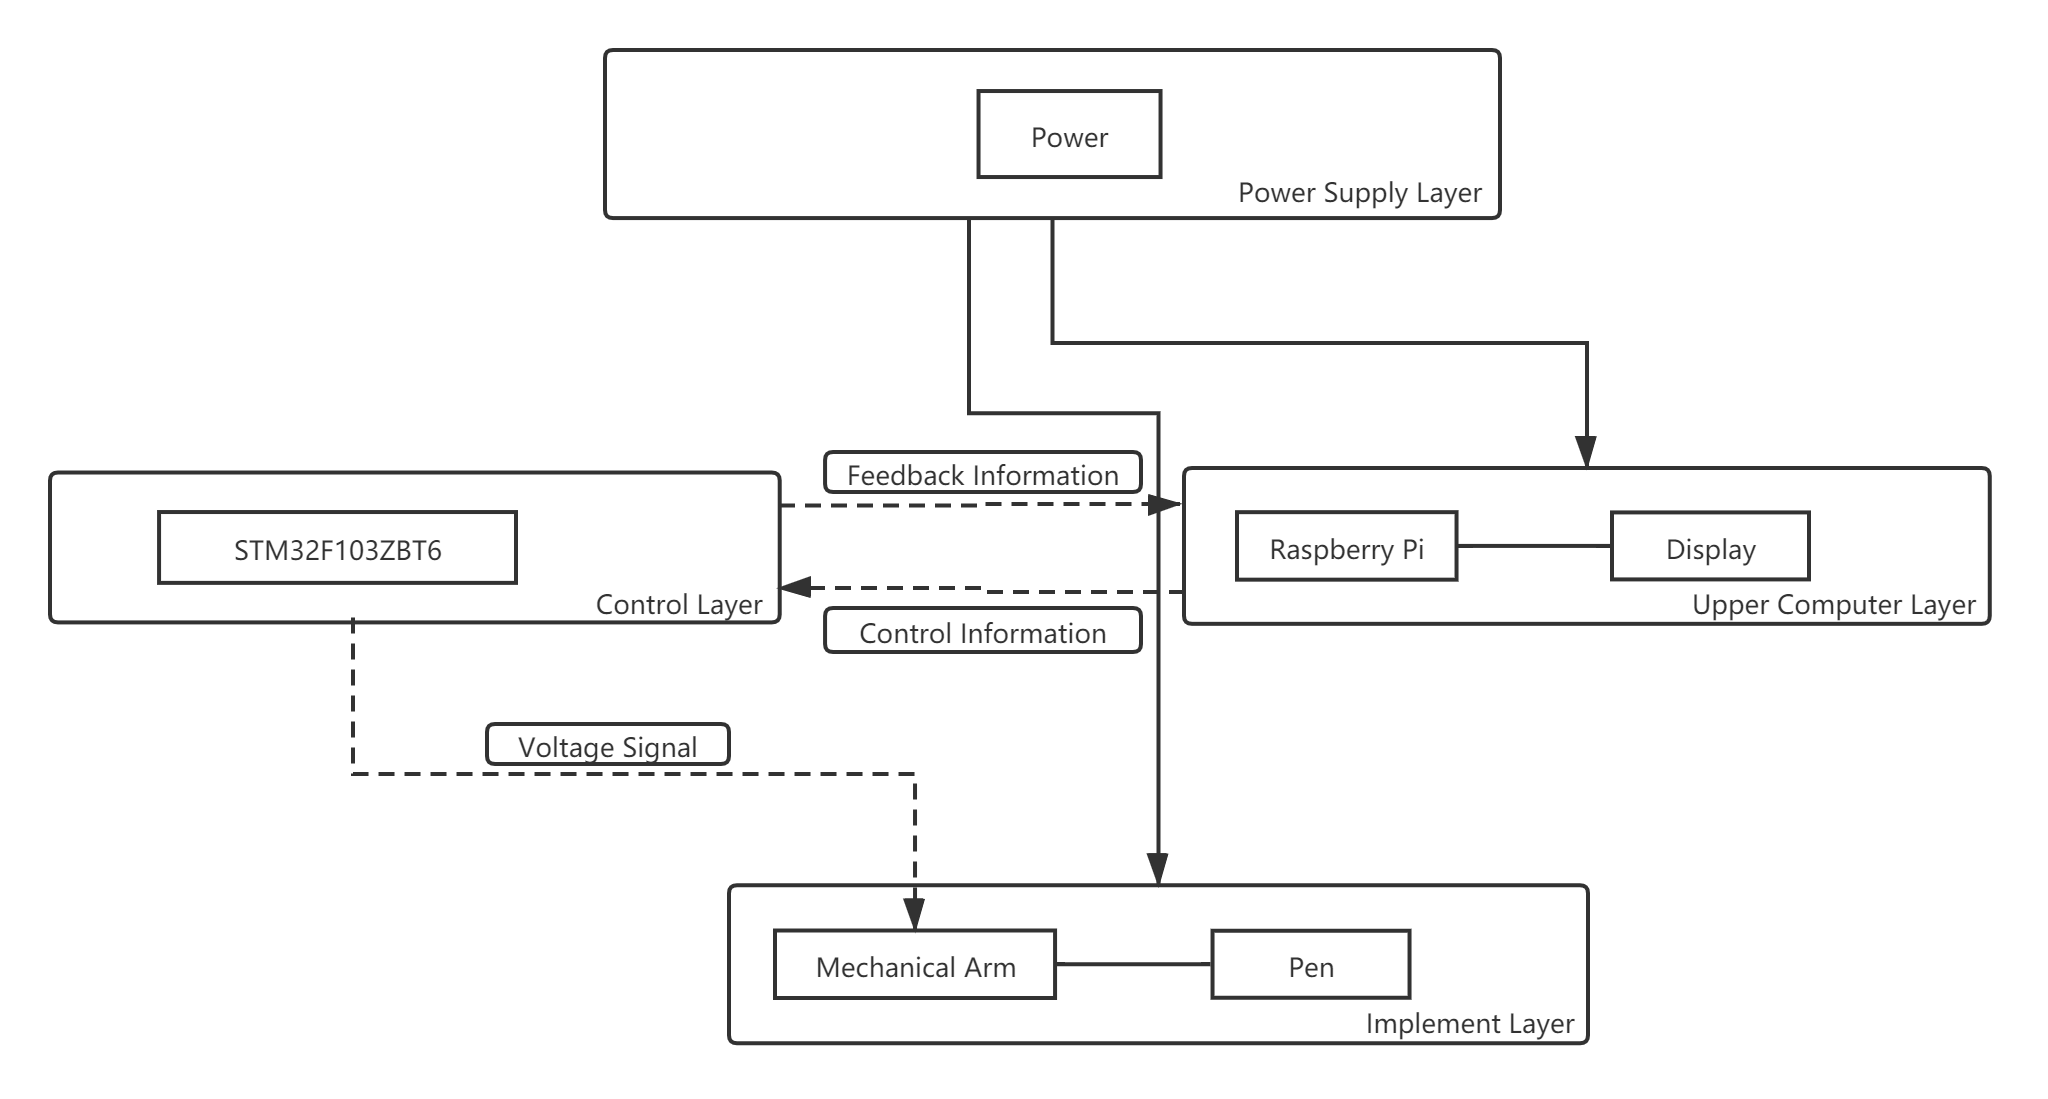
\includegraphics[width=1\linewidth]{figures/HA}
	\caption{Hardware Architecture Diagram}
	\label{fig:HA}
\end{figure}
The hardware structure of the system is shown in the figure1. The system consists of four layers: power supply layer, control layer, upper computer layer and execution layer.

The power supply layer selects the knob power supply as the power supply equipment for the whole system, which supplies the three motors on the manipulator and also supplies power to the raspberry pie.

The upper computer layer is composed of raspberry pie. In this system, the upper computer can send the end target of the end effector of the manipulator. Through the kinematics calculation of the upper computer, the related operations of the three motors are obtained. This information is used as the control information and transmitted to the lower computer through the serial port, that is, the control layer. At the same time, raspberry pie can be connected to the display screen to design gui interface for intuitive operation visualization.

The control layer is composed of motion control board stm32f103zbt6, which connects three motors. The control layer receives the relevant control information (including motor number and rotation angle) sent by the upper computer layer through the serial port, and outputs the pulse signal to control the motor movement. At the same time, the control layer can also send feedback information to the upper computer layer to explain the control effect.

The execution layer is composed of a mechanical arm and a paint barrel. The executive layer receives the voltage signal from the control layer to enable the motor. Under the linkage movement of the three motors, it realizes the control of the paint barrel operated by the end actuator, and realizes the target requirements of the upper computer.

\subsubsection{Software Design}
\begin{figure}[htbp]
	\centering
	
\includegraphics[width=1\linewidth]{figures/SA}
	\caption{Software Architecture Diagram}
	\label{fig:SA}
\end{figure}
The software structure diagram of the system is shown in the figure2. In the system, the upper computer layer and control layer need to carry out software programming.

In the upper computer layer, the system operator inputs the relevant operation information of the manipulator to the upper computer layer in the speech recognition interface or GUI interface. In the upper computer layer, the control information is calculated by kinematics, and the simple control effect is translated into the specific key motion (corresponding to the specific angle of each motor) of the manipulator in order to achieve the motion effect, The specific motion control information is transmitted to the control layer through the serial port and the designed communication protocol.Among them, the voice information is collected through the USB sound card, and can also be input into the voice file prepared locally.

After receiving the motion control information at the serial port, the control layer understands the case according to the designed communication protocol, and then controls the motor motion according to the information.

Through the timer and interrupt software, the PWM pulse signal required for motor motion is output at the GPIO pin. At the same time, the control layer can also feed back the control effect to the upper computer layer through the serial port for GUI display of the control effect.

\subsection{Module List and Module Function Description}
This project is divided into hardware part and software part.
\subsubsection{Hardware Modules}
\begin{table}[htbp] %开始一个表格environment,表格的位置是h,here。  
	\caption{Hardware Core Device Selection} %显示表格的标题
	\centering
	\label{t1}
	\begin{tabular}{c|c} %设置了每一列的宽度,强制转换。 
		\hline
		\hline
		Module& Selection                                                                                                                                         \\
		\hline Motor Driver&A4988 Driver Module\\
		\hline Electric Machinery &42BYH60/47 Two Phase Stepping Motor\\
		\hline	Motion Control Panel&F103ZBT6Stm32 Board\\
		\hline Independent Smart Board&Raspberry Pie 4B\\
		\hline USB Sound Card&Taobao Unknown 19.9yuan Free Shipping\\
		\hline
	\end{tabular}
\end{table}
\begin{itemize}
	\item \textbf{42 series two-phase motor:} Connected with A4988 drive board by motor line. Two 42BYH60 two-phase stepping motors and one 42BYH47 two-phase stepping motor are used as the driving device of the manipulator. The required signal and power supply are provided by A4988 driving board.
	\item \textbf{A4988 drive board:} It is connected with three 42 series two-phase stepper motors through motor lines, and three A4988 drivers are connected with GPIO port of STM32.There are three A4988 drivers on A4988 drive board, corresponding to three stepper motors. Its functions are power supply,set subdivision,STM32 square wave,control direction and speed.In fact, the control speed is to control the pulse frequency, that is, to control the delay time between high and low.When each pulse motor rotates one step, the more pulses per unit time,the greater the rotation angle per unit time,and the faster the speed is.There is a potentiometer on A4988 module, which can adjust the current by turning it.
	\item \textbf{F103ZBT6Stm32:} GPIO port is connected with A4988 driver board, UART serial port is connected with raspberry pie. As a motion control board, three A4988 drivers are connected through the output of GPIO port, and step and dir control signals are generated to control the movement of stepper motor.
	\item \textbf{Raspberry Pie 4B:} As an independent intelligent board, it is connected with the motion control board, namely F103ZBT6Stm32,through the serial port, and completes the tasks of command analysis, path planning and kinematics inverse solution through calculation.
\end{itemize}
The core module selection of the hardware part of this project is shown in Table1.
\begin{figure}[htbp]
	\centering
	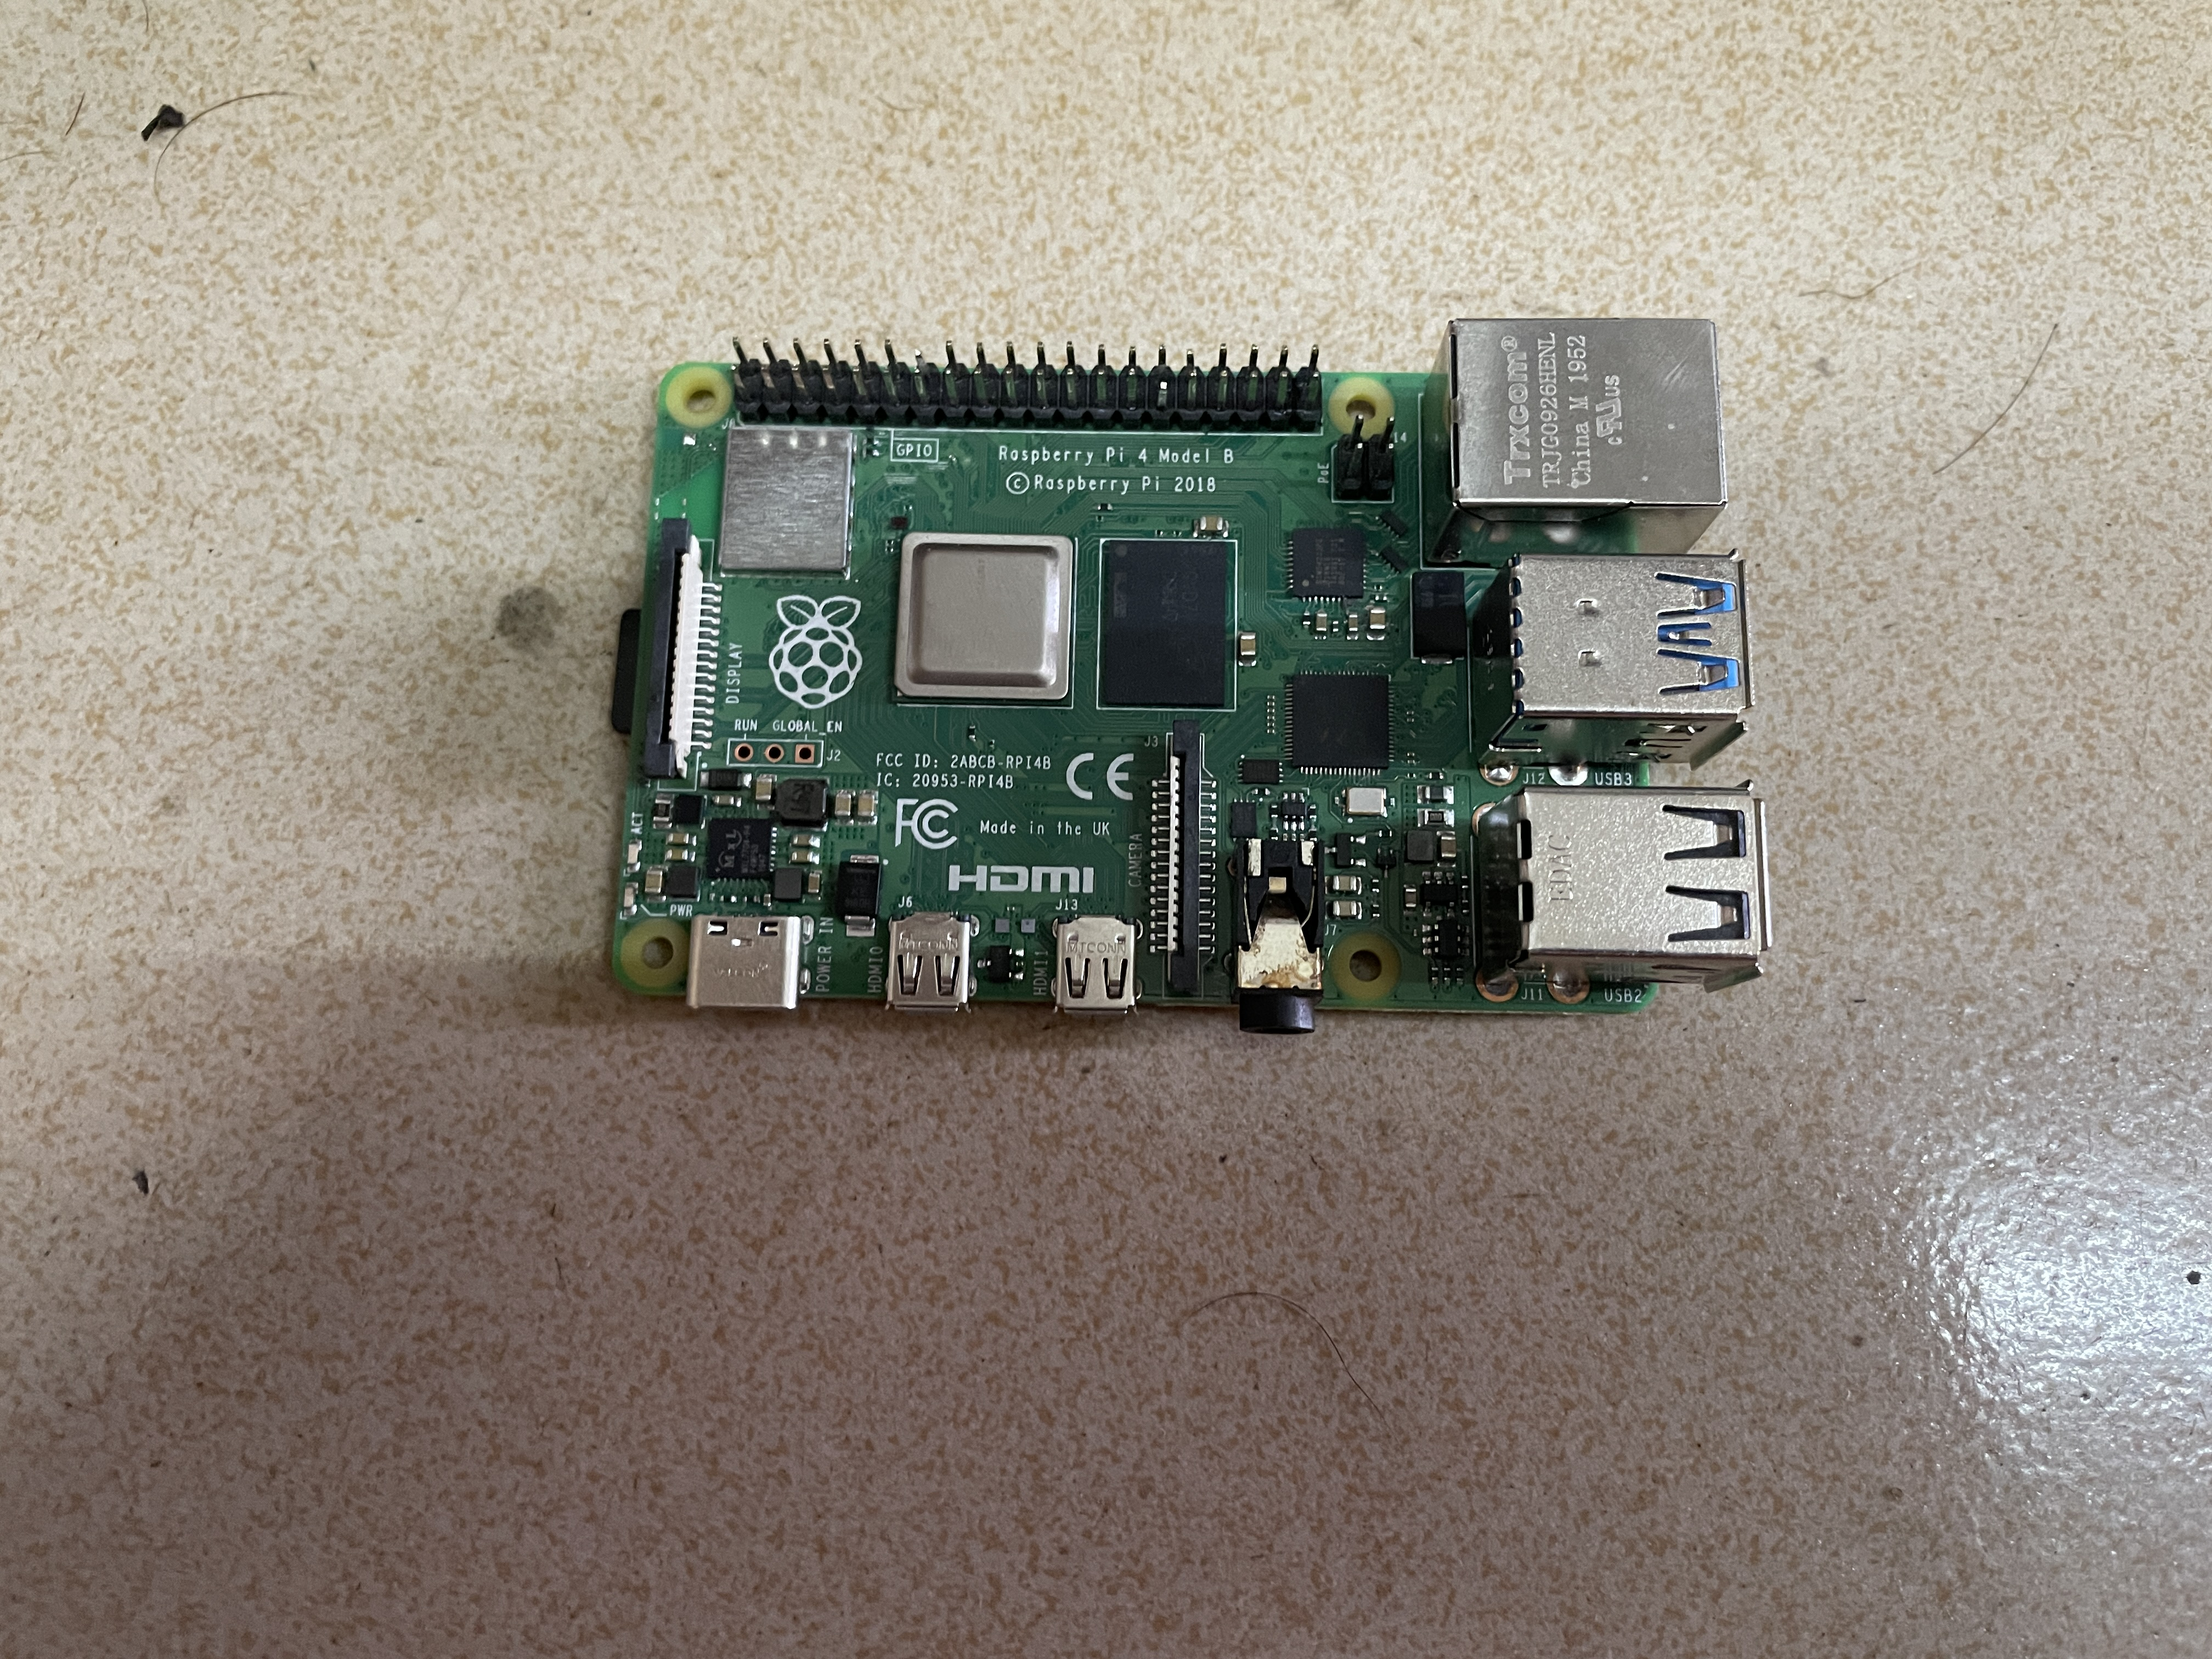
\includegraphics[width=1\linewidth]{figures/RP}
	\caption{Raspberry Pie 4B}
	\label{fig:RP}
\end{figure}
\subsubsection{Software Modules}
The core module selection of the software part of this project is shown in Table2.
\begin{table}[htbp] %开始一个表格environment,表格的位置是h,here。  
	\caption{Software Core Function Description} %显示表格的标题
	\centering
	\label{t2}
	\begin{tabular}{c|p{9cm}} %设置了每一列的宽度,强制转换。 
		\hline
		\hline
		Module Name& Module Function                                                                                                                                         \\
		\hline Upper Computer UI Module&This part is the upper computer of the manipulator, which is completed by the raspberry pie development board with Ubuntu. It mainly realizes the GUI of human-computer interaction, displays the current position of the manipulator, and realizes the interaction with the lower computer.\\
		\hline Trajectory Planning Module&This part is located in the upper computer, which is mainly responsible for trajectory planning. It can realize the interpolation algorithm of straight line, cubic function interpolation of curve and Bessel curve fitting. It is called by the main function of GUI.\\
		\hline	Kinematics Calculation Module&This part is located in the upper computer, which is mainly used as the bridge between GUI and lower computer. Through the kinematics model of the manipulator, the position information needed by the user is transformed into the operation parameters of each joint motor.\\
		\hline	Communication Module&In this part, the communication between the upper computer and the lower computer is realized. The upper computer transmits the operation instructions of the motor to the lower computer, and the lower computer feeds back the state of each joint of the manipulator to the upper computer.\\
		\hline	Motor Drive Module&This part is located in the lower computer, which converts the instructions transmitted by the upper computer into the status of each IO port of the drive motor, and then drives the motor drive board to realize the motor drive.\\
		\hline
	\end{tabular}
\end{table}

\section{Implemented Requirements}

\subsection{Move}
It can move according to the input path within the allowable error range. The software part receives the user's input and performs simple operation in six directions, and the user can adjust the moving speed and single moving distance.

\subsection{Path Planning}
\begin{itemize}
	\item \textbf{MoveJ:}It is the operation of moving one unit, which is the differential unit of the following moveL function.
	\item \textbf{MoveL:}It is a linear moving function. By specifying the coordinates of the end point in the established coordinate system, the manipulator moves linearly from the current position to the target position.
	\item \textbf{MoveP:}It is a function that simulates the function of the palletizer. It simulates a system that grabs all items from one location and moves them to another location for automatic stacking. It can be stacked in multiple layers and is generally used for forklift transportation to warehouse storage.
\end{itemize}
\begin{figure}[htbp]
	\centering
	\includegraphics[width=0.7\linewidth]{figures/B}
	\caption{Single Chip Microcomputer and Control Board}
	\label{fig:B}
\end{figure}
\begin{figure}[htbp]
	\centering
	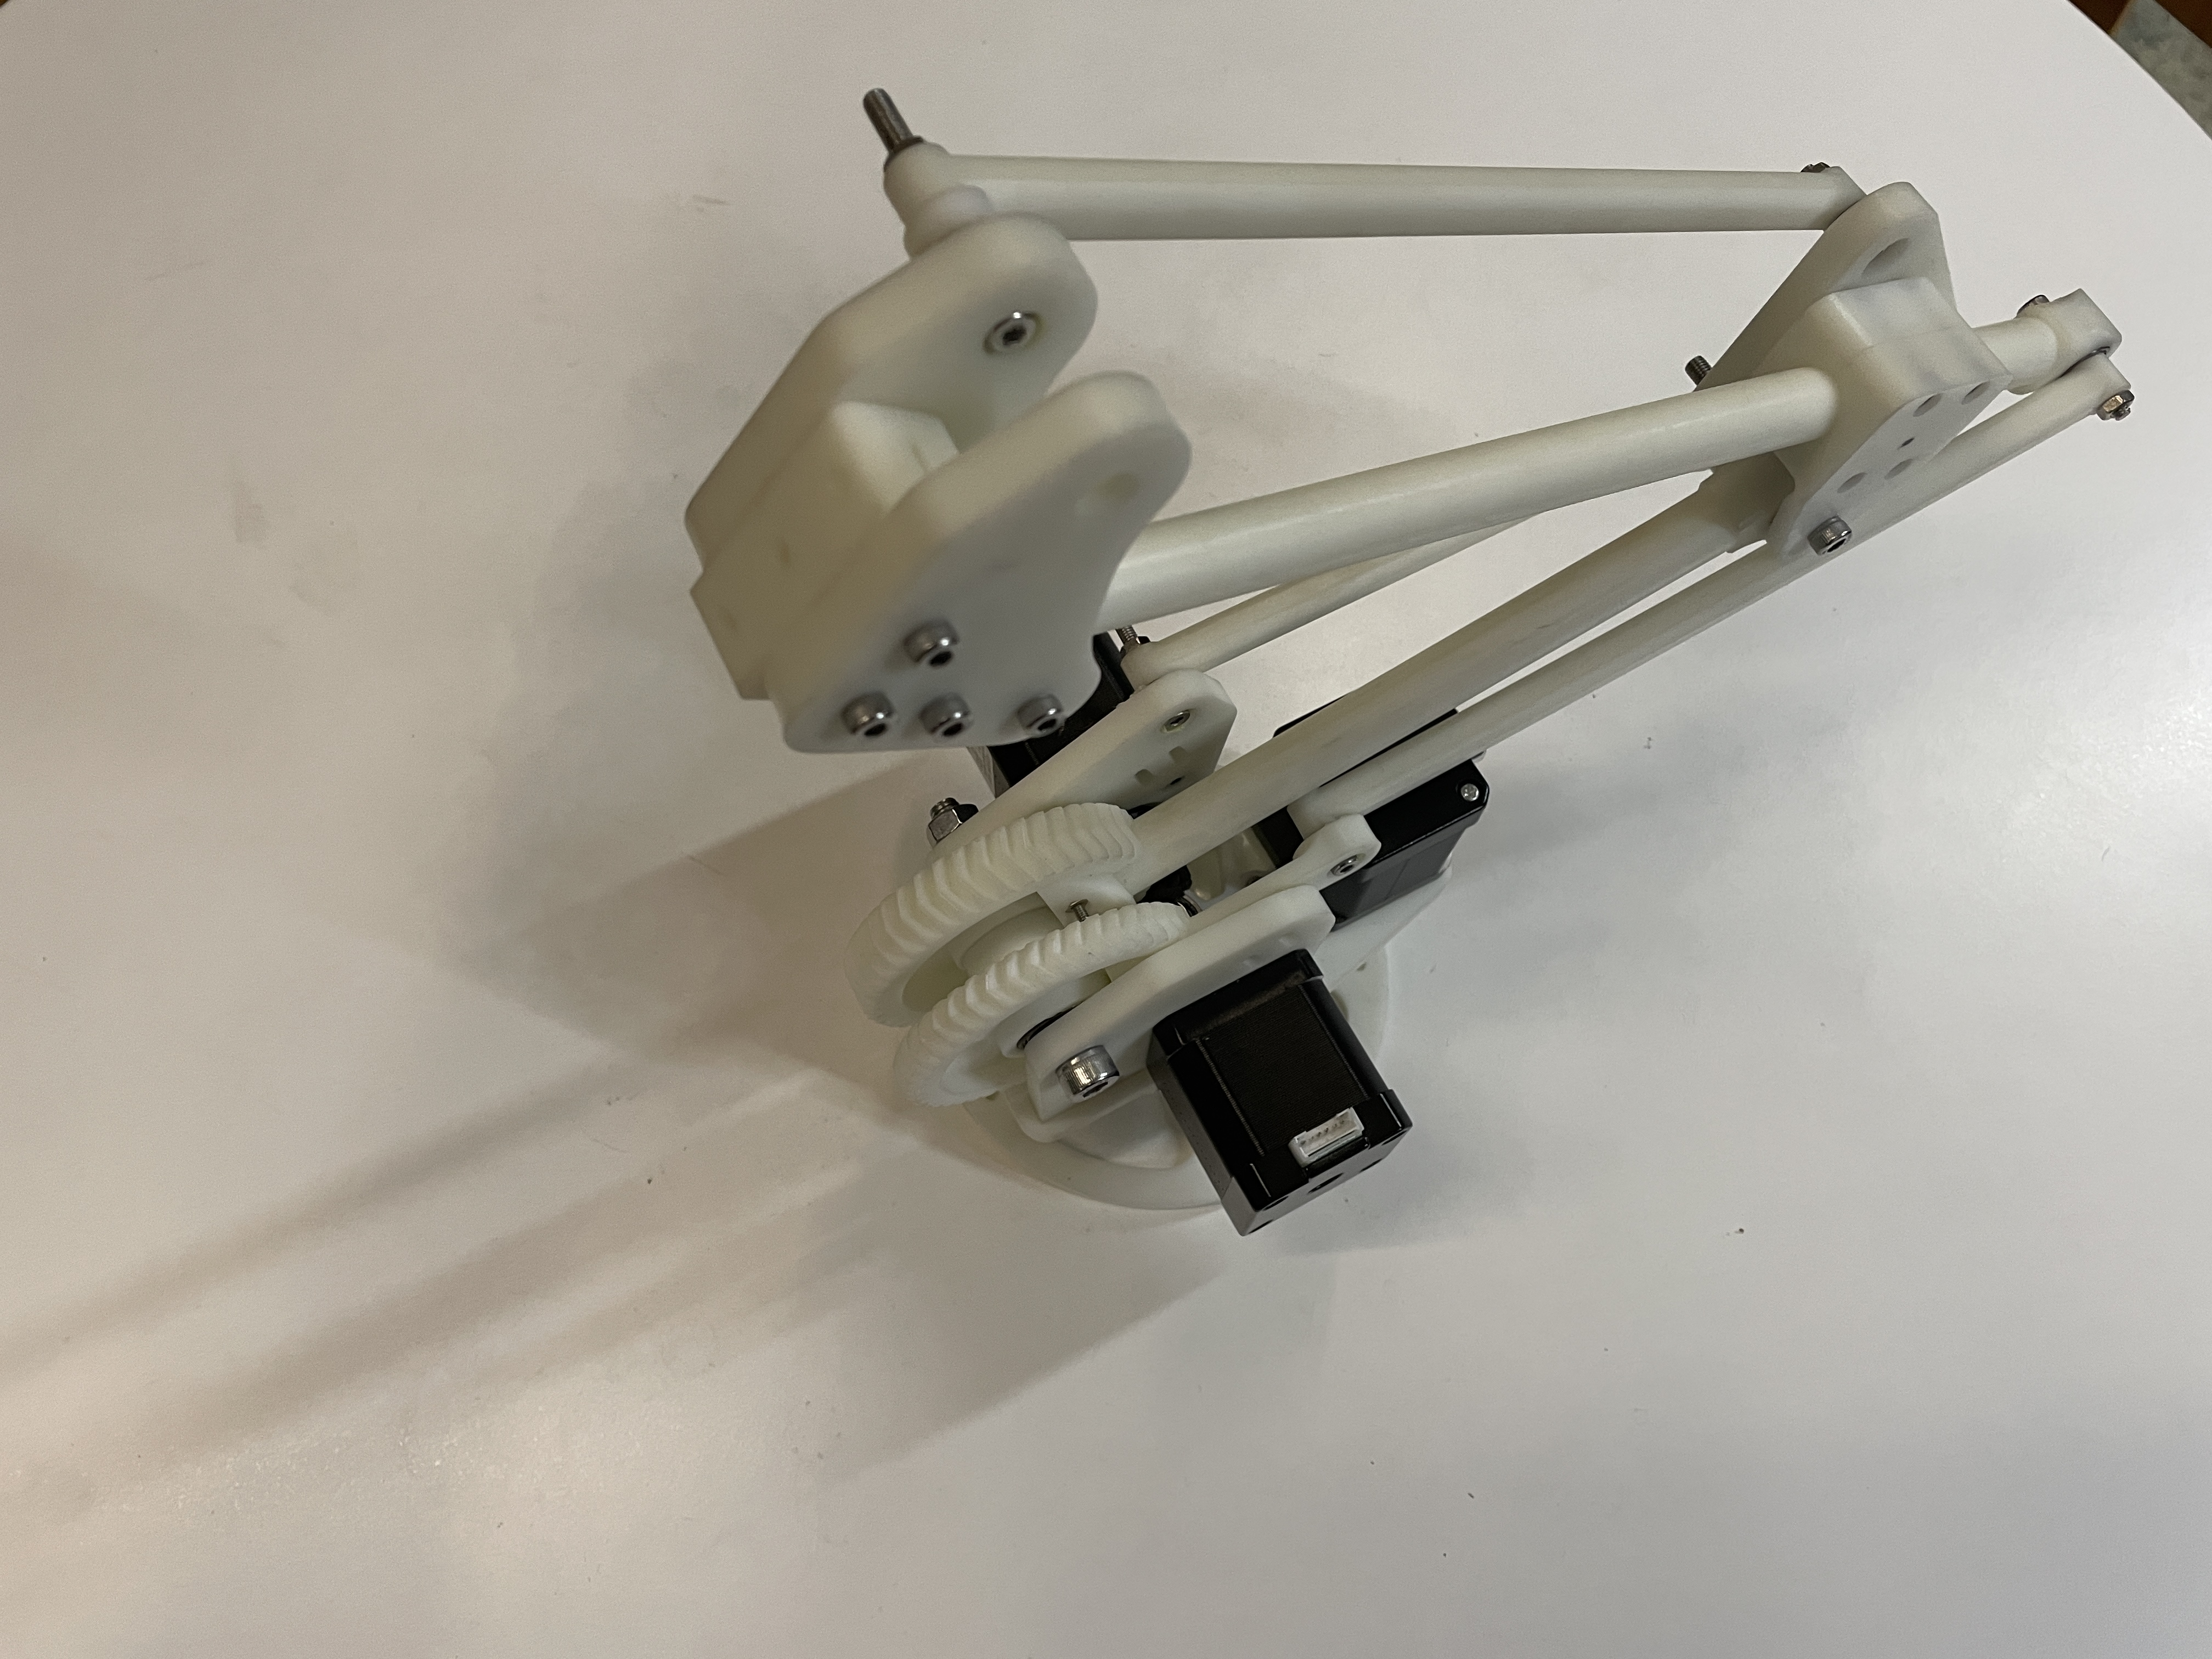
\includegraphics[width=0.7\linewidth]{figures/M}
	\caption{Manipulator}
	\label{fig:M}
\end{figure}
\subsection{GUI}
The system controls the movement of the whole manipulator through the interface. The main functions of the interface are as follows:
\begin{itemize}
	\item Input the coordinates and moving speed of the end effector, and click the end coordinate control button and start button to realize the function of moving the end effector to the input coordinates.
	\item Input the movement direction$(x, y, z)$, the coordinates of the movement distance and the movement speed, and click the single joint control button and start button to realize the function of the manipulator moving a certain distance in the input movement direction.
	\item Input the moving direction $(x, y, z)$, the coordinate of the moving distance and the moving speed, and click the simulate palletizing button and start button to realize the function of simulating palletizing through the curve movement of the manipulator.
	\item Click the up, down, left, right, front, back button and start button to realize the function of the manipulator moving a fixed distance in a certain direction.
	\item Realize the display function of input information of upper computer and feedback information of lower computer in the display text box.
\end{itemize}
\begin{figure}[htbp]
	\centering
	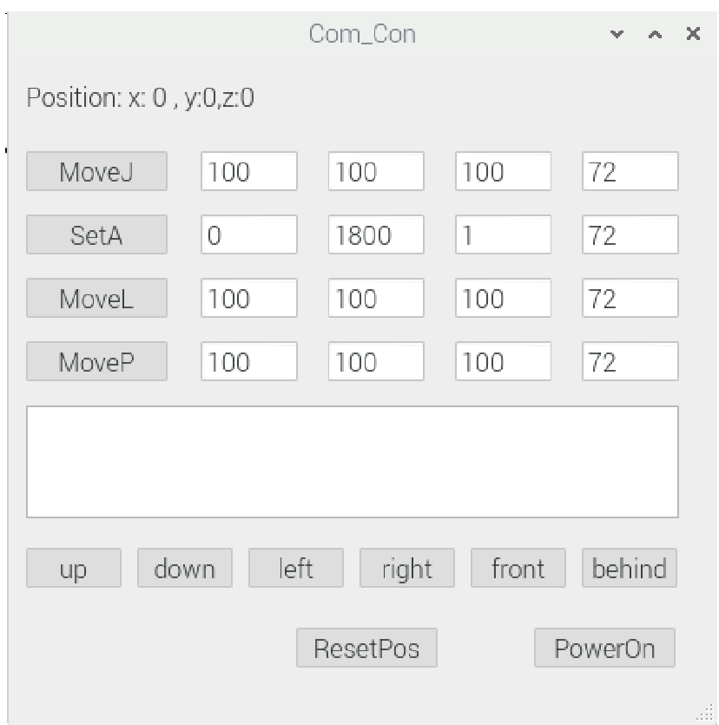
\includegraphics[width=0.7\linewidth]{figures/GUI}
	\caption{Direct Control GUI}
	\label{fig:GUI}
\end{figure}
\subsection{One Click Return}
In some cases, it may be necessary to return to the original position, so we designed a one button return function. By clicking reset on the GUI, we can return the manipulator to its original position.

\subsection{Writing}
In the system, the combined movement mode of numbers and letters is stored, and the robot arm can be controlled to move and write numbers and letters through speech recognition.Detailed examples can be viewed in the submitted video.
\begin{figure}[htbp]
	\centering
	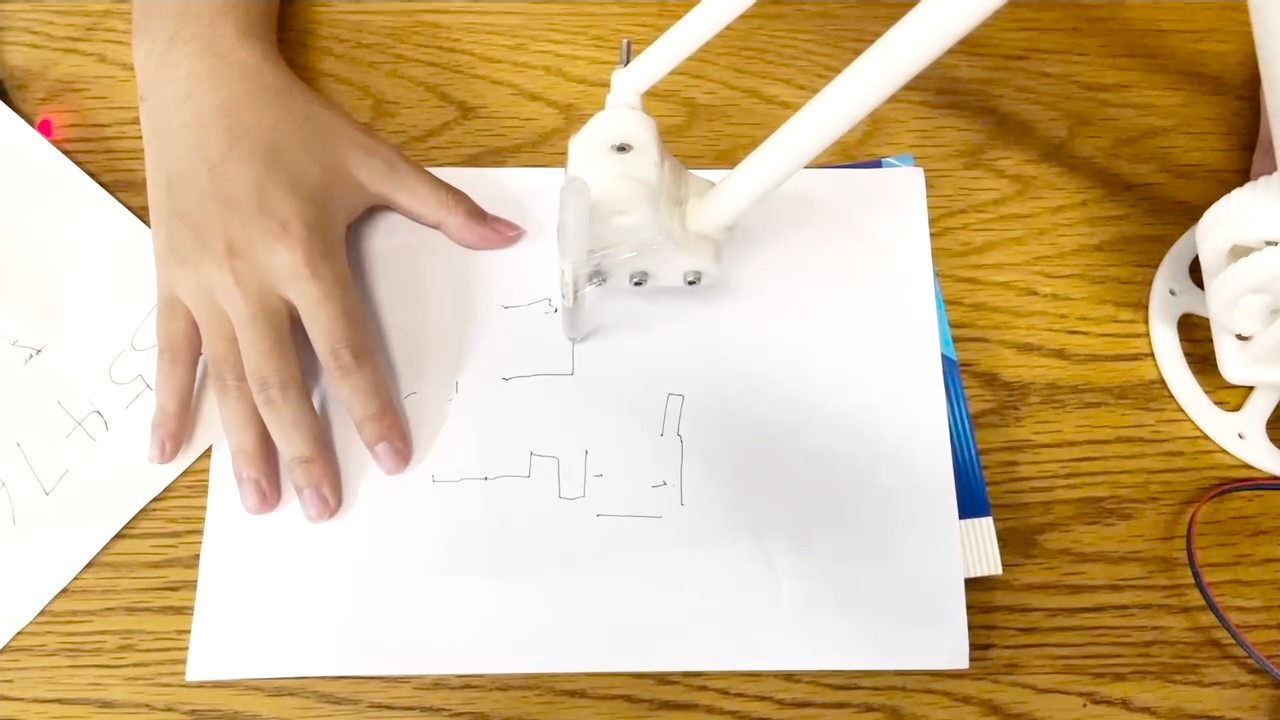
\includegraphics[width=0.8\linewidth]{figures/w1}
	\caption{Writing}
	\label{fig:W}
\end{figure}
\subsection{Palletizing}
After entering the target location, it will plan a curve that does not wipe the ground, then slow down to the highest position, and then move to the target location in the same way. Simulate the process of moving an object by an excavator.
\subsection{Speech Recognition}
The system uses Baidu voice API, which can recognize the user's real-time voice and audio files, and convert the voice into text, so as to control the movement of the manipulator.
This project supports the use of speech recognition function to operate the manipulator movement, the main operations include:
\begin{itemize}
	\item Choose up, down, left, right, front and back six directions to move, you can adjust the moving distance.
	\item Simulate palletizing machine function and plan reasonable path. Complete the simulation of palletizing operation.
	\item According to the user's voice input, write numbers or letters to meet the user's needs.
\end{itemize}
\begin{figure}[htbp]
	\centering
	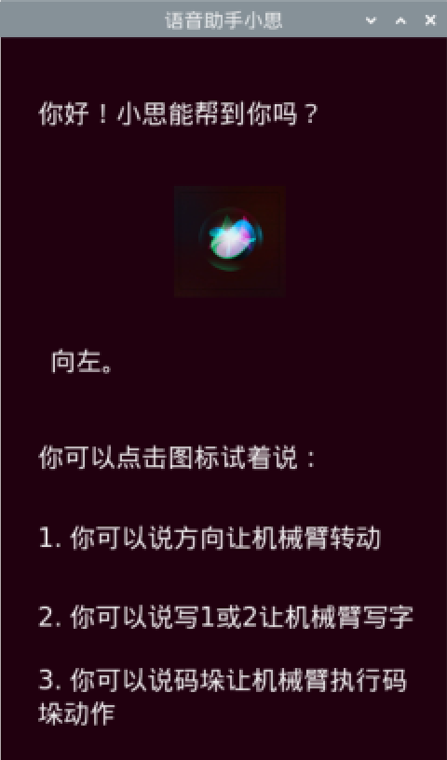
\includegraphics[width=0.5\linewidth]{figures/S}
	\caption{Speech Recognition GUI}
	\label{fig:S}
\end{figure}
We also provide a GUI for speech recognition system, but you need to connect raspberry pi to a monitor to see it. You can't use SSH to connect raspberry pi to see the GUI. A screenshot of the GUI is shown in Figure 7.
\section{Advantages and Disadvantages}
\subsection{Advantages}
\begin{itemize}
	\item Using manipulator instead of manual operation can not only improve the efficiency, but also has a high fault tolerance rate.
	\item The mechanical arm can achieve large-scale mass production, reduce labor costs and technical training costs, optimize cost control, and the product price has market competitiveness.
	\item Professional and technical team can quickly tailor automation solutions according to different product and process requirements of users.
	\item The robot arm has universal design characteristics, which can not only meet the automatic production of "small variety and large batch" workpieces, but also meet the application requirements of "multi variety and small batch".
	\item The mechanical arm is composed of software and hardware, which is highly integrated, high fault tolerance, few fault points and low maintenance cost.
	\item The software system not only develops a simple and beautiful interface, but also provides the function of input speech recognition. The user interaction is very rich.
\end{itemize}

\subsection{Disadvantages}
\begin{itemize}
	\item There is no autonomous mobile capability, and user input is needed to trigger the mobile.
	\item At present, it only supports writing simple numbers and letters, and it is still difficult to write Chinese characters.
	\item The weight of the equipment is not fully considered when making the manipulator. The base of the manipulator is unstable and may fall down.
	\item The wiring of the device is more complicated, and some peripherals such as a monitor, sound card, microphone, mouse, keyboard, etc. are also required.
\end{itemize}

\section{Improvement}
According to the analysis of our advantages and disadvantages, there are many things we can do to improve this program:
\begin{itemize}
	\item The precision error of the X, Y, Z three-axis motion of the manipulator motor is about 0.5cm. After that, experiments and tests can be carried out continuously to optimize the software system, improve the precision, reduce the error and achieve more accurate movement.
	\item At present, the system only supports the writing of letters and numbers, but does not support the writing of complex Chinese characters in mobile programs. This system will continuously improve the software system, and input Chinese characters into the system thesaurus, so that the manipulator can support writing Chinese characters.
	\item At present, the system supports writing on the plane, and then the writing function can be extended to three-dimensional space to complete the writing and description of three-dimensional patterns.
	\item At present, the system supports fixed-point movement, that is, six directions of movement in three-dimensional space, and then can add rotation, expansion and other mobile functions according to the actual needs.
\end{itemize}

\section{Development Environment}
\subsection{Operating System}
\begin{itemize}
	\item \textbf{Windows 10}
	\item \textbf{MacOS}	
	\item \textbf{Linux based on Raspberry Pi}
\end{itemize}
\subsection{Development Tool}
\begin{table}[htbp] %开始一个表格environment,表格的位置是h,here。  
	\caption{Hardware Core Device Selection} %显示表格的标题
	\centering
	\label{DS}
	\begin{tabular}{c|c} %设置了每一列的宽度,强制转换。 
		\hline
		\hline
		Name& Function                                                                                                                                         \\
		\hline VSCode& For integrated development for raspberry pi
		\\
		\hline Baidu Voice API&Speech recognition support
		\\
		\hline	STM32CUBEIDE&For developing embedded C program
		\\
		\hline Qt Designer&For drawing graphical interface\\
		\hline SolidWorks&For kinematics simulation for manipulator\\
		\hline ROS&For kinematics simulation and data output for manipulator\\
		\hline
	\end{tabular}
\end{table}
\subsection{Development Language}
\begin{itemize}
	\item \textbf{Python3.7}
	\item \textbf{C}	
\end{itemize}

\section{Core Code}
The software system part of this project includes several Python scripts. The core code of some scripts is shown below.
\subsection{Change Audio File Sampling Rate}
Using different recording equipment to record the audio file, the file format and sampling rate will be different, and Baidu voice API recognition of the audio file requires the sampling rate must be 16000, this project uses wav audio format, so we need to first use the audio file to WAV format, and the sampling rate to 16000.
\begin{figure}[htbp]
	\centering
	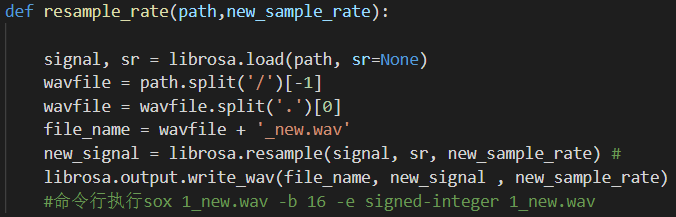
\includegraphics[width=0.9\linewidth]{figures/71}
	\caption{Change Audio File Sampling Rate}
	\label{fig:61}
\end{figure}
\subsection{Move Detailed Data Computing}
According to the needs of users, we can get the distance, angle, speed and terminal position, and convert these data into the data that can be recognized and transmitted by serial communication for serial communication. The manipulator can actually move according to these data to meet the needs of users.
\begin{figure}[htbp]
	\centering
	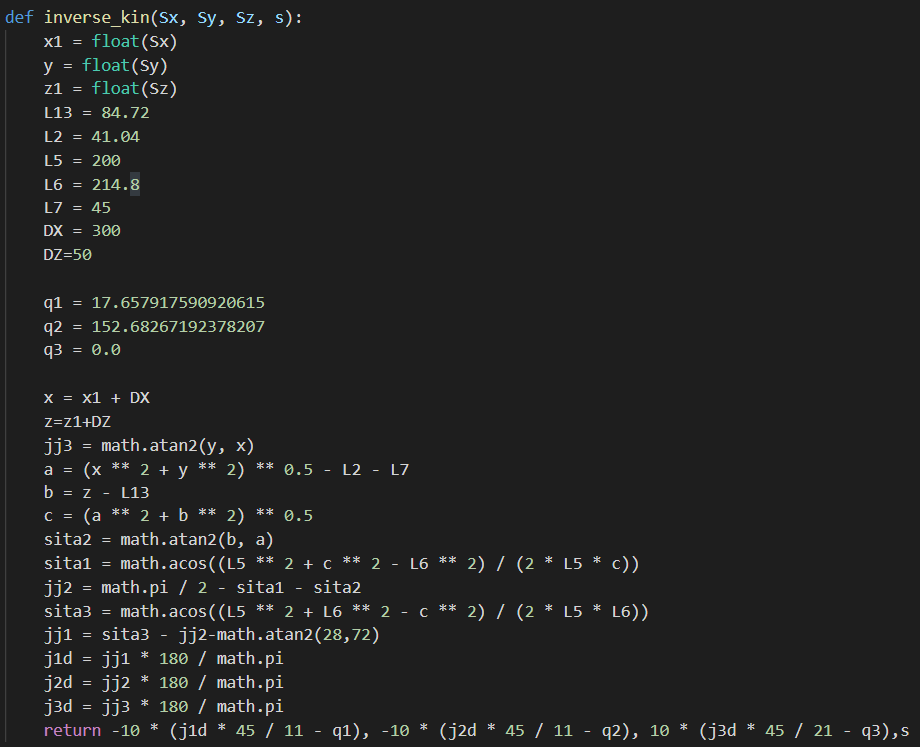
\includegraphics[width=0.9\linewidth]{figures/72}
	\caption{Move Detailed Data Computing}
	\label{fig:62}
\end{figure}
\subsection{User Interface Design}
According to the requirements, we use pyqt to design a user interface, users can choose up, down, left, right, front and back six directions of movement and moving distance, can also select the location of the end point and moving speed to move.
\begin{figure}[htbp]
	\centering
	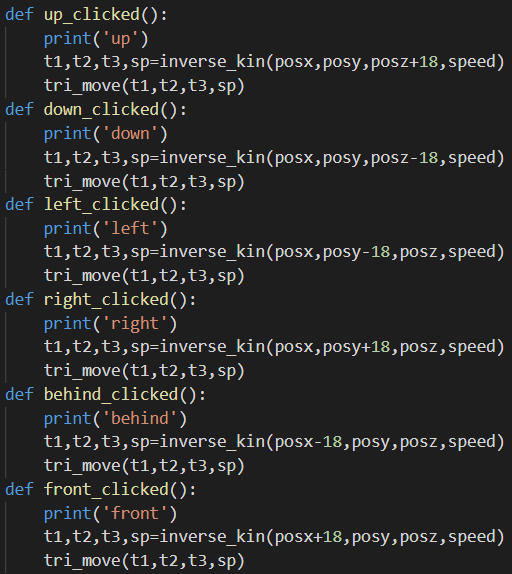
\includegraphics[width=0.9\linewidth]{figures/73}
	\caption{User Interface Design}
	\label{fig:63}
\end{figure}
\begin{figure}[htbp]
	\centering
	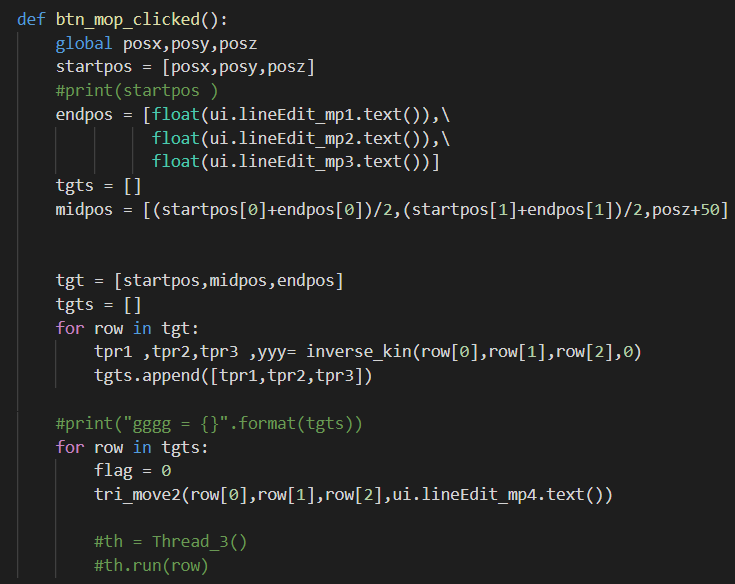
\includegraphics[width=0.9\linewidth]{figures/732}
	\caption{User Interface Design}
	\label{fig:632}
\end{figure}

\subsection{Realization of Speech Recognition}
Users can input voice commands, and the system can recognize voice and make corresponding operations.
\begin{figure}[htbp]
	\centering
	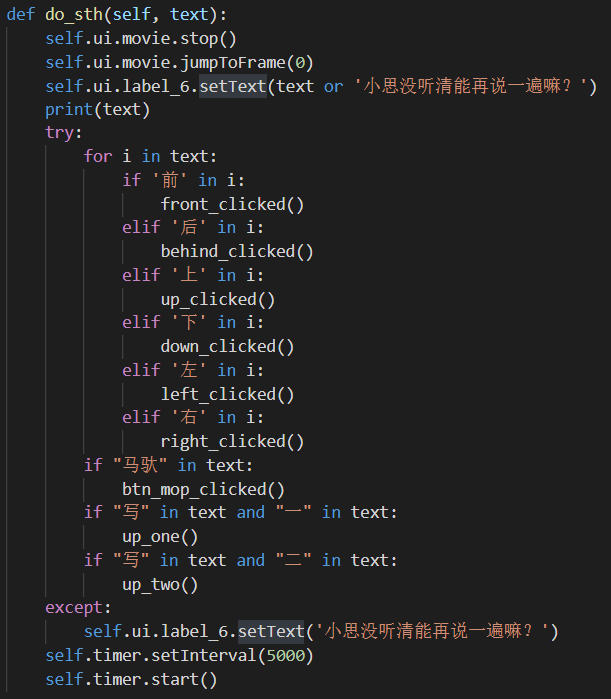
\includegraphics[width=0.9\linewidth]{figures/74}
	\caption{Realization of Speech Recognition}
	\label{fig:64}
\end{figure}

\subsection{Realization of Serial Communication}
Serial communication is the communication function between the software system and the hardware part of the manipulator. The software function transfers a series of mobile data to the hardware, and the hardware makes corresponding mobile operations according to the data.
\begin{figure}[htbp]
	\centering
	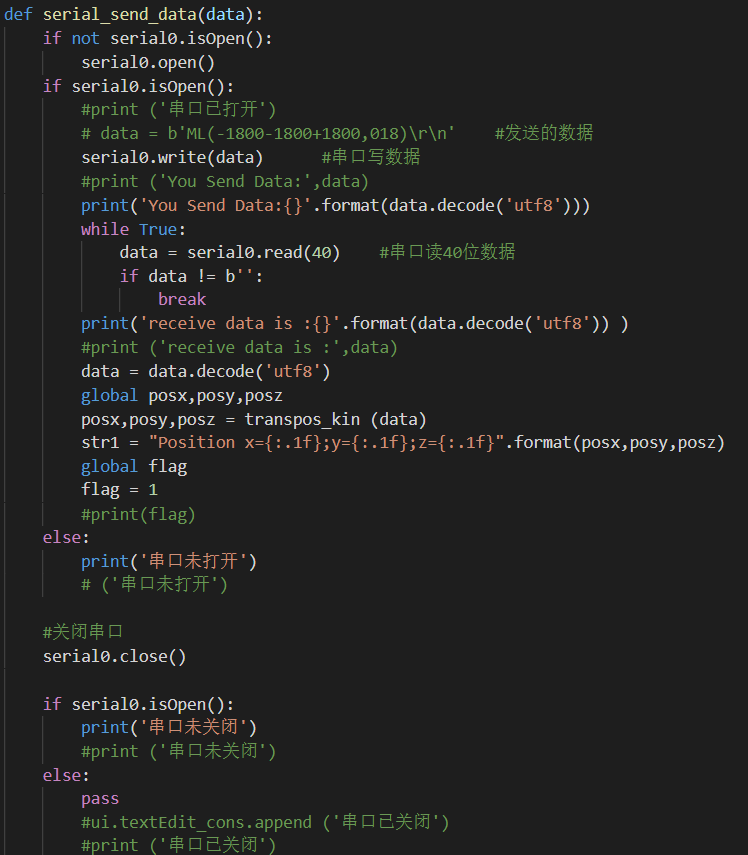
\includegraphics[width=0.9\linewidth]{figures/75}
	\caption{Realization of Serial Communication}
	\label{fig:65}
\end{figure}

\section{Preview Video}
The system running preview video can be seen in the video folder of the submitted file.


\begin{thebibliography}{99}
\bibitem{1} Designing the User Interface: Strategies for Effective Human-Computer Interaction, 6th edition,Ben Shneiderman,Catherine Plaisant,Maxine Cohen
\bibitem{2} Li Hongcheng, Zhang Shuli, Hao Xin, Liu Shenghui. Intelligent control method of desktop manipulator [J]. Technological innovation and application, 2020 (05): 42-43
\bibitem{3} Baidu Speech Recognition Technology Document,\url{https://cloud.baidu.com/doc/SPEECH/index.html}
\end{thebibliography}

\end{document}
%%
%% This work consists of these files mcmthesis.dtx,
%%                                   figures/ and
%%                                   code/,
%% and the derived files             mcmthesis.cls,
%%                  command execution                 mcmthesis-demo.tex,
%%                                   README,
%%                                   LICENSE,
%%                                   mcmthesis.pdf and
%%                                   mcmthesis-demo.pdf.
%%
%% End of file `mcmthesis-demo.tex'.
